\section{Boolean conversion} \label{boolean_conv}
In our datasets, each malware has 119 features, the majority being continuous values. However, as we will see later on with machine learning, some algorithms such as DL8.5 only work on datasets with boolean values. Therefore, these algorithms are limited because only 16 out of the 119 features are boolean. Fortunately, it is possible to convert continuous values into booleans.

For the conversion, we took a dataset of 16 000 pieces of malware that we analysed feature by feature. We will show a conversion example with feature number 16, which corresponds to the headers feature, but the same reasoning was applied to all features. 

\begin{enumerate}
    \item \textbf{Distribution analysis:} when we look at the distribution of values on figure \ref{fig:fv_repartition}, we can observe that:
    \begin{figure}[!h]
        \centering
          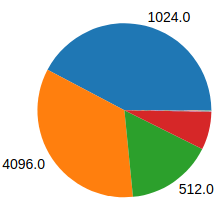
\includegraphics[width=0.30\linewidth]{Figures/fv_repartition.png}
          \caption{Distribution of the values of feature 16}
          \label{fig:fv_repartition}
        \end{figure}

    \begin{itemize}
        \item 42\% takes the value 1024 (in blue)
        \item 34\% takes the value 4096 (in orange)
        \item 16\% takes the value 512 (in green)
        \item 7\% takes the value 1536 (in red)
        \item 1\% has a different value than those listed above - the proportion is represented between red and blue.
    \end{itemize}
    
    \item \textbf{Bucketing:} This mechanism converts continuous values into discrete ones. For example, if a feature corresponds to the age of a person, it can take a value between 0 and 105. We can therefore convert this value into the \textit{young}, \textit{adult} and \textit{old} categories to limit our possibilities to 3 instead of 105. In the case of our problematic, we keep the 4 most present values and gather the "others" in one value.
    
    We choose: 
    \begin{itemize}
        \item 1 for 1024.
        \item 2 for 4096.
        \item 3 for 512.
        \item 4 for 1536.
        \item 0 for others values.
    \end{itemize}
    
    \item \textbf{One-hot encoding:} Now that the possibilities are limited, we convert these values into booleans using one-hot encoding. In this case where we have 5 possibilities, one feature is sprayed upon 5 features which will have the \textit{true} or \textit{false} in the corresponding column. Table \ref{tab:a_onehot} shows the values for three malware before the one-hot encoding and their resulting conversion is indicated in table \ref{tab:b_onehot}.
    
    \begin{table}[!h]
        \centering
        \begin{tabular}{|c|c|}
            \hline
             MalwareID &  F16 \\
             \hline
             1 & 3 \\
             \hline
             2 & 0 \\
             \hline
             3 & 4 \\
             \hline
        \end{tabular}
        \caption{Value of feature 16 for three malware before one-hot encoding}
        \label{tab:b_onehot}
    \end{table}
    
    \begin{table}[!h]
        \centering
        \begin{tabular}{|c|c|c|c|c|c|}
            \hline
             MalwareID &  F16\_0 &  F16\_1 & F16\_2 & F16\_3 & F16\_4  \\
             \hline
             1 & 0 & 0 & 0 & 1 & 0 \\
             \hline
             2 & 1 & 0 & 0 & 0 & 0 \\
             \hline
             3 & 0 & 0 & 0 & 0 & 1 \\
             \hline
        \end{tabular}
        \caption{Resulting values of feature 16 for 3 malware after one-hot encoding}
        \label{tab:a_onehot}
    \end{table}
\end{enumerate}

One disadvantage of this technique is the rapid increase in terms of number of features, which is why it is absolutely necessary to efficiently limit the number of possibilities when bucketing.

\section{Normalisation and standardisation}

As said in the previous section, the 119 features used in our ground truths can have pretty much any range of values. While some models might tolerate such disparity, other computations need the data to fit within a specific interval. This is for example the case for distance-based algorithms. They use the distance between points to compute specific measures, such as deviation from normality as in \cite{ugarte-pedrero_structural_2011}. If the data does not use the same scale, there is a chance that higher weights are given to features with higher magnitudes, impacting the performance of the algorithms. Mechanisms such as normalisation and standardisation can then be used such that all features are equally treated. Long story short, normalisation scales data between 0 and 1 while standardisation does it within the [-1,1] interval.

Since these pre-processing steps are linked to machine learning and specific to the type of model used, they will be more deeply explained and illustrated in section \ref{first_phase}.